\chapter{The Ising Model, Mean Field, and the First Phase Transition}

These notes follow Leonard Susskind's ninth lecture on statistical mechanics. The aim is not to solve the Ising model in every dimension, but to understand, in a mathematically controlled way, why one dimension has no phase transition while higher dimensions do. Where the blackboard captures a key equation or construction, the preserved frames from LazyingArt LLC and Video2Book are kept as visual evidence alongside a cleaned reconstruction.

\section{Ising Revisited and Today's Problem}

Susskind opens by repairing a historical injustice. Ising did \emph{not} fail to solve the one-dimensional model. He solved it correctly, and he correctly found that the one-dimensional Ising model has no phase transition. The mistake came afterward: on the basis of that result he concluded that the Ising model has no phase transition in \emph{any} dimension. That is the point that fails.

So the lecture begins with a very clear target. We are not going to solve the higher-dimensional Ising models exactly; they are too hard. What we are going to do instead is use an approximation that is simple enough to calculate with and physical enough to trust when the number of neighbors is large. In that approximation we will see a genuine phase transition: a sudden change in the behavior of the system as the temperature is varied.

But Susskind does not jump straight to the approximation. He resets the problem first. Let us go back to the simplest magnet we already understand, recover the basic \(\tanh\) formulas, and then climb from there.

\section{One Spin in a Heat Bath}

The warm-up is a single two-state magnet. We write
\begin{equation}
\sigma=\pm 1,
\end{equation}
with \(\sigma=+1\) meaning up and \(\sigma=-1\) meaning down. Susskind simplifies the notation from the previous lecture by absorbing the magnetic moment and the magnetic field into one parameter \(j\), and he chooses the sign convention
\begin{equation}
E=-j\,\sigma.
\end{equation}
For \(j>0\), the lower-energy state is the up state.

Instead of treating a whole collection of such spins at once, we now regard one spin as a subsystem in equilibrium with the rest of the magnet, which acts as a heat bath. The one-spin partition function is then
\begin{align}
z
&=\sum_{\sigma=\pm1} e^{-\beta E(\sigma)}
 =\sum_{\sigma=\pm1} e^{\beta j\sigma} \\
&= e^{\beta j}+e^{-\beta j}
 =2\cosh(\beta j).
\end{align}
This is the same simple system as before, but in a form that we will soon reuse twice: once for the bond variables in one dimension, and once again in mean field.

The blackboard preserves the next step particularly clearly.

\begin{figure}[ht]
\centering

\includegraphics[width=0.78\textwidth]{lecture_09_figure_02.png}
\caption{One-spin average energy reduced to hyperbolic tangent form.}
\end{figure}

From the partition function,
\begin{align}
\langle E\rangle
&=-\frac{\partial}{\partial\beta}\log z
 =-\frac{1}{z}\frac{\partial z}{\partial\beta} \\
&=-j\,\frac{\sinh(\beta j)}{\cosh(\beta j)}
 =-j\,\tanh(\beta j).
\end{align}
Since the energy is just \(-j\) times the spin, we can read off the average spin immediately:
\begin{equation}
\langle \sigma\rangle=\tanh(\beta j).
\end{equation}
Susskind also calls this the magnetization of the simple magnet.

This formula already contains the temperature story in embryo. The function \(\tanh x\) has slope \(1\) at the origin, tends to \(1\) for large positive \(x\), and tends to \(-1\) for large negative \(x\). So when \(\beta j\) is large and positive, the spin is almost certainly up; when \(\beta j\) is near zero, the average spin is near zero; and if we reverse the sign of \(j\), the whole graph simply flips. Very high temperature destroys the bias. Low temperature reveals it sharply.

\section{The One-Dimensional Ising Model and the Question of Memory}

Now we turn to the next magnet in the hierarchy: the one-dimensional Ising chain. At each site \(i\) there is a spin \(\sigma_i=\pm1\), and the energy of the whole chain is
\begin{equation}
E=-j\sum_i \sigma_i\sigma_{i+1}.
\end{equation}
The minus sign makes parallel neighbors favorable, so for \(j>0\) the lowest-energy states are the two fully aligned ones: all spins up or all spins down.

Susskind also notes that if we changed the sign of \(j\), the mathematics in one dimension would not really change. By flipping the sign of every other spin we would convert the antiferromagnetic-looking problem back into the ferromagnetic one. So we keep the minus sign and the aligned ground states.

The central question, however, is not merely what the ground state is. The real question is whether one spin can influence another arbitrarily far away. Suppose we know that a spin at one site is up. What can we say about a spin \(n\) links down the chain? In the lecture this is framed first as a conditional-probability question and then recast in the standard language of correlation functions:
\begin{equation}
\langle \sigma_i \sigma_{i+n}\rangle.
\end{equation}
If this quantity stays nonzero at large distance, the chain has long-range memory. If it dies away, then the bias from one spin eventually gets lost. This is the first real diagnostic of magnetization in the interacting system: does the information carried by one spin survive to infinity, or not?

\section{Bond Variables, Factorization, and Correlation Decay}

What is the trick? The trick, as Susskind puts it, is a marvelous one: do not focus on the spins, focus on the links between them.

Take an open chain of \(N\) spins. We first fix the first spin, say \(\sigma_1=+1\), and restore the other choice later by a factor of \(2\). Now define the bond variables
\begin{equation}
\mu_i=\sigma_i\sigma_{i+1}, \qquad i=1,\dots,N-1.
\end{equation}
Each \(\mu_i\) is again \(\pm1\). It records whether the neighboring spins are parallel or anti-parallel.

Once \(\sigma_1\) is fixed, the \(\mu_i\) determine the whole chain. Indeed,
\begin{equation}
\sigma_{i+1}=\sigma_i\,\mu_i,
\end{equation}
and iterating gives
\begin{equation}
\sigma_{i+n}=\sigma_i\,\mu_i\mu_{i+1}\cdots\mu_{i+n-1}.
\end{equation}
So there is no loss of information: sites have been traded for bonds.

The reward is immediate, because the energy becomes
\begin{equation}
E=-j\sum_{i=1}^{N-1}\mu_i.
\end{equation}
The interacting spin chain has been rewritten as a sum over independent bond variables. For the sector with \(\sigma_1=+1\),
\begin{align}
Z_{\uparrow}
&=\sum_{\{\mu_i=\pm1\}}
\exp\!\left(\beta j\sum_{i=1}^{N-1}\mu_i\right) \\
&=\prod_{i=1}^{N-1}\left(\sum_{\mu_i=\pm1} e^{\beta j\mu_i}\right) \\
&=[2\cosh(\beta j)]^{N-1}.
\end{align}
Restoring the two choices of the first spin gives
\begin{equation}
Z=2[2\cosh(\beta j)]^{N-1}.
\end{equation}
There is one fewer bond than spin, which is why the exponent is \(N-1\).

This is the exact one-dimensional solution in the form Susskind wants. The problem has reduced to the same one-spin calculation as before, but the meaning of the degree of freedom has changed. The variable is no longer a magnet at a site; it is the relation between two neighboring magnets.

The nearest-neighbor correlation is therefore exactly the one-spin answer again:
\begin{equation}
\langle \mu_i\rangle=\tanh(\beta j),
\end{equation}
so
\begin{equation}
\langle \sigma_i\sigma_{i+1}\rangle=\tanh(\beta j).
\end{equation}
At infinite temperature, \(\beta=0\), even this nearest-neighbor correlation vanishes.

To get the long-distance correlation, we now choose a clean convention: \(n\) will mean the number of bonds between the two spins. Then
\begin{align}
\langle \sigma_i\sigma_{i+n}\rangle
&=\left\langle \mu_i\mu_{i+1}\cdots\mu_{i+n-1}\right\rangle \\
&=\langle \mu_i\rangle \langle \mu_{i+1}\rangle \cdots \langle \mu_{i+n-1}\rangle \\
&=[\tanh(\beta j)]^n.
\end{align}
Because \(|\tanh(\beta j)|<1\) at every finite temperature, the correlation falls exponentially with distance. This is the exact mathematical statement of Susskind's ``telephone game'' analogy: each step down the chain costs another factor of fidelity.

\subsection{Question \& Answer}

The lecture pauses over a natural objection.

If the correlation function is just \(\langle \sigma_i\sigma_{i+n}\rangle\), why is it legitimate to insert all those intermediate factors?

Because we are inserting nothing but \(1\)'s:
\begin{equation}
1=\sigma_{i+1}^2=\sigma_{i+2}^2=\cdots=\sigma_{i+n-1}^2.
\end{equation}
Thus
\begin{align}
\sigma_i\sigma_{i+n}
&=\sigma_i(\sigma_{i+1}^2)(\sigma_{i+2}^2)\cdots(\sigma_{i+n-1}^2)\sigma_{i+n} \\
&=(\sigma_i\sigma_{i+1})(\sigma_{i+1}\sigma_{i+2})\cdots(\sigma_{i+n-1}\sigma_{i+n}) \\
&=\mu_i\mu_{i+1}\cdots\mu_{i+n-1}.
\end{align}
Nothing has been altered. We have only rewritten the quantity of interest in terms of the variables for which the measure factorizes.

Susskind also remarks that this is already a little duality: a theory of coupled site variables has been converted, by a clever change of variables, into a theory of uncoupled bond variables.

\section{From Telephone to Mean Field in Higher Dimensions}

The one-dimensional chain is therefore, in Susskind's word, a boring system. It is magnetized only at absolute zero. At any finite temperature there is some loss of fidelity, and once a mistake is made the next site has no support system. It hears only from one direction. That is why long stretches of agreement occur, but genuine long-range memory does not survive.

Now we pivot. Instead of playing telephone along a line, suppose each site hears from many directions. In two dimensions a site on a square lattice has four nearest neighbors; in three dimensions it has six; in \(d\) dimensions it has \(2d\). If one message is wrong but three are right, the site can use a majority rule. In the language Susskind borrows from computer science, it can perform error correction. That is the new physical mechanism.

The point of considering large \(d\) is not that we live in ten thousand spatial dimensions. It is that a hard problem often becomes transparent in a limit. If a spin has many neighbors, the bias in the sum of those neighbors is of order \(2d\), while the fluctuation is only of order \(\sqrt{2d}\). Large numbers invite averaging. Once we understand the limit, we can ask where the new behavior first appears. In the Ising model, the answer is already between one and two dimensions.

That motivates the mean-field approximation. Focus on one distinguished spin \(\sigma\). Its exact local energy is
\begin{equation}
E_{\text{local}}=-j\,\sigma\sum_{\text{neighbors}}\sigma_{\text{neighbor}}.
\end{equation}
The blackboard introduces this from left to right: geometry, then local energy, then the average spin.

\begin{figure}[ht]
\centering

\includegraphics[width=0.76\textwidth]{lecture_09_figure_03.png}
\caption{Local spin energy in two dimensions before mean-field replacement.}
\end{figure}

The sketch is only schematic, so it helps to redraw the intended picture cleanly.

\begin{figure}[ht]
\centering
\begin{tikzpicture}[scale=1.15]
\fill (0,0) circle (2pt);
\draw (0,0) -- (1.4,0);
\draw (0,0) -- (-1.4,0);
\draw (0,0) -- (0,1.4);
\draw (0,0) -- (0,-1.4);
\draw (1.4,0) circle (0.08);
\draw (-1.4,0) circle (0.08);
\draw (0,1.4) circle (0.08);
\draw (0,-1.4) circle (0.08);
\node at (0,0.28) {$\sigma$};
\end{tikzpicture}
\caption{A clean schematic of one chosen spin and its nearest-neighbor environment in two dimensions.}
\end{figure}

Now suppose the lattice has average spin \(\bar{\sigma}\), which from this point on we identify with \(\langle \sigma\rangle\). Mean field replaces the fluctuating neighbor sum by its average value:
\begin{equation}
\sum_{\text{neighbors}}\sigma_{\text{neighbor}}
\;\longrightarrow\;
2d\,\bar{\sigma}.
\end{equation}
Then
\begin{align}
E_{\text{local}}
&=-j\,\sigma\sum_{\text{neighbors}}\sigma_{\text{neighbor}} \\
&\longrightarrow -2dj\,\bar{\sigma}\,\sigma
=:E_{\text{mf}}.
\end{align}

\begin{figure}[ht]
\centering

\includegraphics[width=0.78\textwidth]{lecture_09_figure_04.png}
\caption{Mean-field replacement of the neighbor sum by an average spin.}
\end{figure}

This is now just the one-spin problem again, but with an effective field created by the other spins. If we temporarily denote the average of the distinguished spin by \(\bar{\bar{\sigma}}\), then the one-spin calculation gives
\begin{equation}
\bar{\bar{\sigma}}=\tanh(2\beta d j\,\bar{\sigma}).
\end{equation}
But the distinguished spin is not special. Translation invariance tells us that its average should be the same as the average of every other spin. Therefore
\begin{equation}
\bar{\bar{\sigma}}=\bar{\sigma},
\end{equation}
and we arrive at the self-consistency condition
\begin{equation}
\bar{\sigma}=\tanh(2\beta d j\,\bar{\sigma}).
\end{equation}

\begin{figure}[ht]
\centering

\includegraphics[width=0.78\textwidth]{lecture_09_figure_05.png}
\caption{Self-consistent equation for the average spin.}
\end{figure}

\subsection{Question \& Answer}

At this point the lecture fields two closely related questions.

Is the final \(\bar{\sigma}\) outside the \(\tanh\), and is the bar notation the same thing as an average?

Yes to the second, no to the first. Susskind explicitly says he is simply switching from angle brackets to an overbar, so \(\bar{\sigma}\) means the average spin. And the self-consistency equation is genuinely implicit:
\begin{equation}
\bar{\sigma}=\tanh(2\beta d j\,\bar{\sigma}),
\end{equation}
with \(\bar{\sigma}\) \emph{inside} the argument of the hyperbolic tangent. The chalk spacing in the isolated board equation momentarily makes it look as if a factor might sit outside, but the lecture immediately corrects that reading.

\begin{remark}
The approximation is justified only when \(d\) is large enough that the average of the \(2d\) neighbors dominates their fluctuation. Susskind says this more than once: the formula is not to be taken seriously in low dimension merely by plugging in \(d=1\).
\end{remark}

\section{Self-Consistency, the Graphical Solution, and the Phase Transition}

How do we solve the implicit equation, and how do we see the physics in it? Susskind's answer is to simplify the argument of the \(\tanh\) first. Define
\begin{equation}
y=2\beta d j\,\bar{\sigma}.
\end{equation}
Then the self-consistency equation becomes
\begin{equation}
\frac{y}{2\beta d j}=\tanh y.
\end{equation}

\begin{figure}[ht]
\centering

\includegraphics[width=0.78\textwidth]{lecture_09_figure_06.png}
\caption{Reduced transcendental equation before the graphical solution.}
\end{figure}

Now the problem has become geometric. The right-hand side is the fixed curve \(\tanh y\). The left-hand side is a straight line through the origin with slope
\begin{equation}
\frac{1}{2\beta d j}.
\end{equation}
If we prefer to write \(T=1/\beta\), the same slope is \(T/(2dj)\). Susskind makes that shift in language on the board so that the temperature itself appears as the control parameter.

At very high temperature the line is steep, and the only intersection with \(\tanh y\) is at the origin. Therefore the only self-consistent solution is
\begin{equation}
\bar{\sigma}=0.
\end{equation}
That is exactly what we expect: high temperature randomizes the spins.

As the temperature is lowered, the line rotates downward. The critical moment occurs when the line is tangent to \(\tanh y\) at the origin. Since
\begin{equation}
\tanh'(0)=1,
\end{equation}
the critical condition is
\begin{equation}
\frac{1}{2\beta_c d j}=1,
\end{equation}
or equivalently
\begin{equation}
2\beta_c d j=1.
\end{equation}
In temperature language,
\begin{equation}
T_c=2dj.
\end{equation}
Below this temperature the line is shallower than the tangent, and new nonzero intersections appear. Those correspond to states with nonzero average magnetization.

\begin{figure}[ht]
\centering
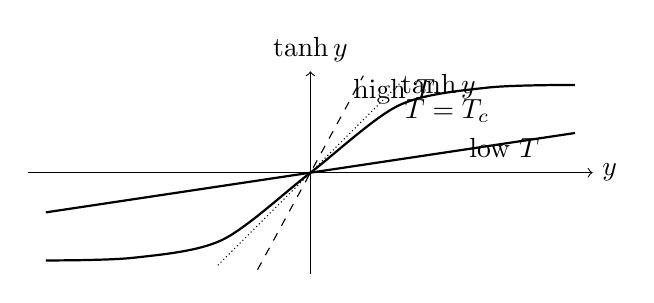
\begin{tikzpicture}[scale=1.12]
\draw[->] (-3.2,0) -- (3.2,0) node[right] {$y$};
\draw[->] (0,-1.15) -- (0,1.15) node[above] {$\tanh y$};

\draw[smooth,thick]
plot coordinates {(-3,-0.995) (-2,-0.964) (-1,-0.762) (0,0) (1,0.762) (2,0.964) (3,0.995)};

\draw[dashed] (-0.6,-1.1) -- (0.6,1.1);
\draw[densely dotted] (-1.05,-1.05) -- (1.05,1.05);
\draw[thick] (-3,-0.45) -- (3,0.45);

\node at (1.45,0.98) {$\tanh y$};
\node at (0.95,0.92) {high \(T\)};
\node at (1.55,0.70) {\(T=T_c\)};
\node at (2.2,0.28) {low \(T\)};
\end{tikzpicture}
\caption{Graphical solution of \(\frac{y}{2\beta d j}=\tanh y\). High temperature gives only the origin, the critical line is tangent there, and low temperature produces nonzero branches.}
\end{figure}

This is the first appearance of the phase transition in the lecture. A branch with \(\bar{\sigma}=0\) exists at high temperature, and a magnetized branch appears when the slope passes through the critical value.

\subsection{Question \& Answer}

But now wait a minute: even below the transition, the origin is still an intersection of the two curves. How do we know that the physical solution is not the one at the origin?

Susskind does not brush this question away. He handles it in two stages. First, he notes that if we start from zero temperature, where alignment is beyond doubt, and then raise the temperature, the aligned state must continue along the nonzero branch until the transition is reached. Second, he promises a sharper answer by turning on a tiny external magnetic field. Before doing that, however, the lecture takes up another objection: why one should not trust the same mean-field formula at \(d=1\).

\section{Why \(d=1\) Fails, and How a Tiny Field Picks a Branch}

\subsection{Question \& Answer}

What goes wrong if we simply put \(d=1\) into the mean-field equation?

The short answer is that the mean-field argument only made sense when the number of neighbors was large. The deeper answer comes from looking at low-temperature excitations.

Go first to absolute zero. Then everybody wants to align. Now increase the temperature slightly and ask what new configurations enter the partition function. In two dimensions, flipping one spin breaks four bonds. If we flip a larger compact region, the energy cost grows with the length of its boundary. The more spins we flip, the more broken bonds we typically create.

In one dimension the geometry is radically different. Flip one spin and we break two bonds. Flip two adjacent spins and we still break only two bonds. Flip three adjacent spins, or ten, or a hundred, and the energy cost is still the energy of two broken bonds. In other words,
\begin{equation}
\Delta E_{1d}(\text{one contiguous flipped block})
=\text{energy of two broken bonds},
\end{equation}
independent of the block length, whereas in two dimensions
\begin{equation}
\Delta E_{2d}(\text{flipped droplet})\propto \text{boundary length}.
\end{equation}

That is the missing physics. In one dimension, long reversed domains are entropically cheap: there are many of them, and they cost no more energy than short ones as long as they remain contiguous. Susskind phrases this concretely. The number of configurations with a fixed extra energy in one dimension is very large, because one may choose any two bonds and flip every spin in between. That count grows like the square of the number of sites. In two dimensions, by contrast, the energy keeps rising as the flipped region grows. That is why one dimension is unstable to large flipped segments as soon as the temperature is turned on.

So the mean-field formula does not fail because some algebraic singularity appears at \(d=1\). It fails because the approximation has thrown away precisely the geometrical feature that distinguishes one dimension from higher dimensions.

\subsection{Question \& Answer}

Now return to the earlier question. The origin is still a formal solution below the transition. How do we decide which branch is physical?

We add a tiny external magnetic field. The lecture fumbles the sign briefly on the board, so let us choose a clean convention: positive \(b\) favors up spins. Then the mean-field energy of one spin becomes
\begin{equation}
E_{\text{mf},b}=-2dj\,\bar{\sigma}\,\sigma-b\,\sigma.
\end{equation}
The one-spin calculation therefore gives
\begin{equation}
\bar{\sigma}=\tanh(2\beta d j\,\bar{\sigma}+\beta b).
\end{equation}
Keeping the same definition \(y=2\beta d j\,\bar{\sigma}\), we get
\begin{equation}
\frac{y}{2\beta d j}=\tanh(y+\beta b).
\end{equation}
The left-hand side has not changed. The right-hand side is the same \(\tanh\) curve shifted horizontally. Equivalently, one may keep the \(\tanh y\) curve fixed and think of the family of straight lines as acquiring a nonzero intercept. The lecture discusses both viewpoints live on the board.

Either way, the origin is no longer a solution. Once \(b\neq0\), however small, the symmetry between the two magnetized branches is broken. For \(b>0\), the branch with positive magnetization is preferred. Then, at fixed temperature below the critical one, we may let \(b\to0^+\) and remain on that branch. The zero-magnetization solution is therefore not the physically stable one; it is an unstable symmetric solution.

This is Susskind's concrete version of spontaneous symmetry breaking. A state with average zero may exist formally as a fifty-fifty balance between up and down, but in a macroscopic system the tiniest bias is enough to choose a direction. The field can be arbitrarily small, yet the total energy difference between an up-oriented and a down-oriented sample is enormous because the number of spins is enormous. That is why a real ferromagnet does not remain indecisive once it is placed even in a weak ambient field.

\section{Summary}

The lecture unfolds in three movements. First we rebuild the one-spin problem and recover the basic hyperbolic-tangent formulas. Then we solve the one-dimensional Ising chain exactly by changing variables from spins to bonds, and we learn that
\begin{equation}
\langle \sigma_i\sigma_{i+n}\rangle=[\tanh(\beta j)]^n,
\end{equation}
so long-range memory dies exponentially at every finite temperature. Finally we turn to higher dimension, where many neighbors make averaging plausible, and mean field leads to the self-consistency equation
\begin{equation}
\bar{\sigma}=\tanh(2\beta d j\,\bar{\sigma}).
\end{equation}
Its graphical solution shows a critical temperature,
\begin{equation}
T_c=2dj,
\end{equation}
below which magnetized branches appear.

What one dimension lacked was not coupling but support. Domains of reversed spins are too cheap there. In higher dimension the boundary cost of a flipped region grows, and long-range order can survive. A tiny external field then picks one magnetized branch and reveals the instability of the symmetric zero-average state. That is the lecture's payoff: the Ising model becomes the first sharp example in which memory, geometry, and phase transition can all be seen in one connected argument.